\documentclass[submit,techrep,noauthor]{ipsj}

% \usepackage[dvips]{graphicx}
\usepackage[dvips,dvipdfmx]{graphicx}
\usepackage{url}
% \usepackage{graphicx}
% \usepackage[dvipdfmx]{color}
\usepackage{caption}
\usepackage{tabularx}
\newcolumntype{Y}{>{\arraybackslash}X}
\usepackage{latexsym}
% \usepackage{hyperref}

\usepackage{listings,jlisting}
\lstset{
  basicstyle={\ttfamily},
  identifierstyle={\small},
  commentstyle={\textit},
  keywordstyle={\small\bfseries},
  ndkeywordstyle={\small},
  stringstyle={\small\ttfamily},
  frame={tb},
  breaklines=true,
  columns=[l]{fullflexible},
  numbers=left,
  xrightmargin=0zw,
  xleftmargin=3zw,
  numberstyle={\scriptsize},
  stepnumber=1,
  numbersep=1zw,
  lineskip=-0.5ex
}
\renewcommand{\lstlistingname}{listing}


\begin{document}

\affiliate{cs}{筑波大学大学院理工情報生命学術院システム情報工学研究群情報理工学位プログラム}
\affiliate{ccs}{筑波大学計算科学研究センター}

\title{CA VOL: HDF5におけるコンテキストによるI/O最適化}

\author{木下 嵩裕}{Kinoshita Takahiro}{CS}[kinoshita@hpcs.cs.tsukuba.ac.jp]
\author{建部 修見}{Osamu Tatebe}{CCS}[tatebe@cs.tsukuba.ac.jp]

\begin{abstract}
	HPCにおけるアプリケーションの多くはHDF5やnetCDF等の高レベルI/Oライブラリを利用してI/O処理を行う.
	HDF5には,Virtual Object Layer(VOL)という機能があり,高レベルなAPIでI/O処理を置き換える仕組みがある.
	既存のI/Oでは,このVOLの中で利用可能であるデータの型のサイズ,データのレイアウト等のコンテキストを活用できていない.
	本研究では,このVirtual Object Layerで得ることのできるコンテキストを活用することで,I/O処理の最適化を行うVOLプラグインCA VOLを提案する.
	コンテキストを元にデータの書き込み境界とファイルシステムでのチャンクサイズを合わせ,I/Oの並列度を高めることで,I/Oを高速化した.
\end{abstract}

\maketitle

\section{はじめに}
近年,HPCでは,計算機の性能が指数関数的に向上している.
しかし,演算器の性能向上と比較して,ストレージの性能向上は計算機の性能向上に追いついていない.
特に,現代のシミュレーションサイズの増加に伴い,ストレージ性能の不足がシステムのボトルネックとなっている.
このストレージとの性能の乖離へ対処するために,
グローバルファイルシステムとのキャッシュストレージの研究,不揮発メモリといった新たなデバイスの開発が進んでいる.

キャッシュストレージ層,新しいストレージデバイスが登場することにより,
ストレージレイヤーはより複雑になっている.
このような複雑なストレージレイヤーやデバイスの特性を意識することなく
効率的にアプリケーションを実行できることが求められており,
ストレージ中間層\cite{wang2016burstbuffer,moody2017unifyfs},
ad-hocファイルシステム~\cite{vef2018gekkofs,tatebe2022chfs}の研究がされている.


多くのHPCアプリケーションは,HDF5\cite{hdf5}やpnetCDF\cite{pnetcdf}等高レベルI/Oライブラリを利用してI/O処理を行う.\cite{byna2020exahdf5}
これらの高レベルI/Oライブラリの内部のI/O処理には,MPIO実装であるROMIOという低レベルI/Oライブラリが採用されている.
ROMIOはMPIによるIOを抽象化するレイヤーであり,LustreやGPFSなどのファイルシステムに対しての実装が用意されている.
特定のサイズの大量データの連続書き込みにおいては高速だが,特定のアクセスパターンや小規模データセット,stridedなアクセス,ランダムアクセスが多い場合
その性能は著しく低下する.

HDF5などの高レベルI/OライブラリはMPIOを利用してI/O処理を行うが,
呼び出される際,MPIIOはデータの書き込みコンテキストなどの情報を十分に利用できていない.
また,HDF5には,Virtual Object Layer(VOL)という機能がある.
このVirtual Object Layerを活用したI/O処理について,
Huihuo Zengらによる計算ノードのローカルSSDを利用した研究\cite{zheng2022hdf5}.
Jerome Sounmagneらによる分散オブジェクトストレージであるDAOSを使った研究がある\cite{soumagne2021accelerating}.
これらの研究では,Virtual Object Layerの実装で得ることのできる情報を活用しきれていない.
このVirtual Object Layerで得られるコンテキストを活用することで,I/O処理への活用が期待される.

高レベルI/Oライブラリを利用していることによって得られる,
そのI/Oがどの機能によって発生したのか,
書き込みはどの位置でどのサイズか,などの書き込みコンテキストを活用できていない.
ストレージ層を意識せずに高いI/O性能を得るために,
この書き込みコンテキストの活用が必要である.


\begin{figure}[t]
	\centering
	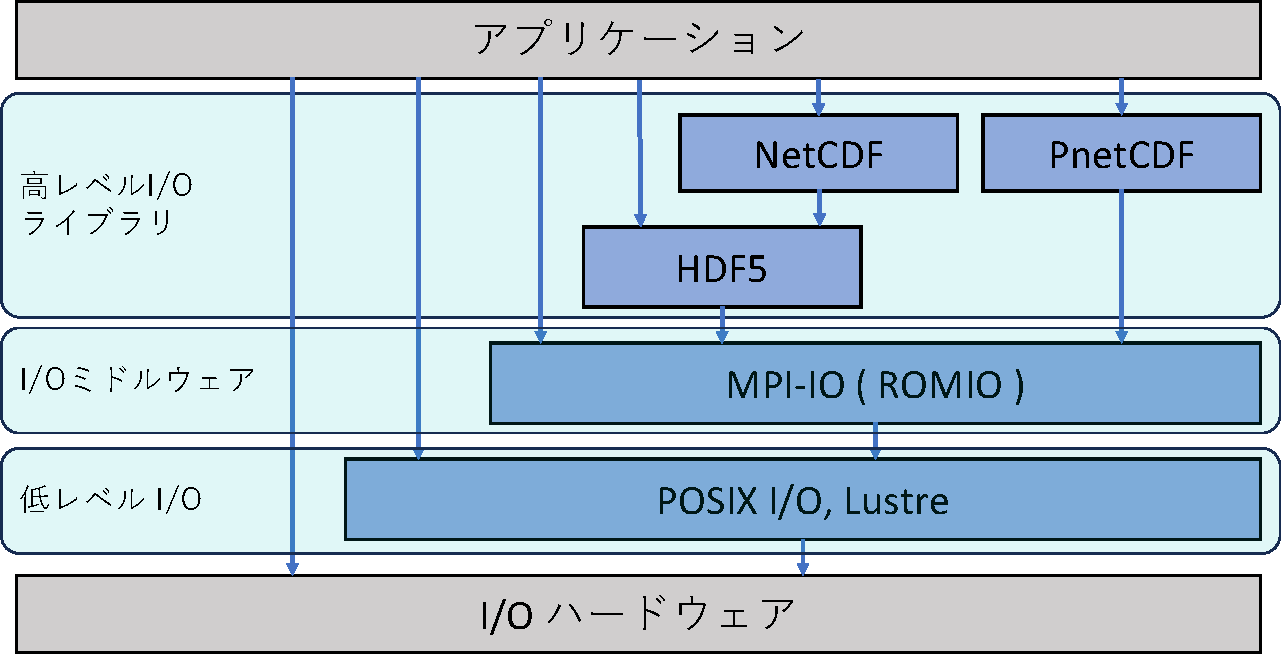
\includegraphics[page=1,width=\linewidth]{figure-crop.pdf}
	\caption{HPCのIOスタック}
	\label{fig:iotstack}
\end{figure}


\section{関連研究}

HDF5のVirtual Object Layerを用いてI/Oを高速化するシステムに関する研究は多く行われている.

Huihuo Zengらによる計算ノードのローカルSSDを利用した研究がある\cite{zheng2022hdf5}.
この研究では,Read時はHDF5のファイルをアドレス空間にまずマップする.
そのアドレス空間を分割し,同期,非同期的に各ノードで担当アドレス空間の部分を共有ファイルシステムから読み込む.
他のノードからの読み込みが発行された際には,その担当ノードに対してReadを発行し読み込みの高速化をする.
Read時のシステムの構成図を\figref{fig:cachevolread}に示す.

機械学習などの計算時間よりも読み込み時間が多いシステムにおいては,
並列共有ファイルシステムからの読み出しがボトルネックとなることが多い.
このキャッシュによって,I/O時間の削減ができる.
また,Write時には,各ノードのSSDに一時的に書き込み,
その後,非同期で共有ファイルシステムに書き戻す.
それによりPOSIXセマンティクスは満たさないものの,
プログラムから見える実効速度はノードローカルSSDのものになるため,
高速なI/Oの実現が可能である.
この非同期による書き込みの操作はJerome Soumagneらによる
Async VOL\cite{tang2021transparent}という非同期I/OをするVOLプラグインが利用されている.
Write時のシステムの構成図を\figref{fig:cachevolwrite}に示す.
この研究ではノードローカルストレージを透過的に利用することで高速化を実現している.
しかし,この研究ではHDF5のVirtual Object Layer中で得ることができるコンテキストを
活用できていない.

\begin{figure}[t]
	\centering
	\includegraphics[page=6,width=\linewidth]{figure-crop.pdf}
	\caption{DAOS VOLの構成}
	\label{fig:voldaos}
\end{figure}

Jerome Sounmagneらによる分散オブジェクトストレージであるDAOSを使った研究がある\cite{soumagne2021accelerating}.
DAOSは分散Key-Value storeであり,高いスケーラビリティを持つことが特徴である.
この研究では,HDF5のデータをKey-Value Storeで格納できるように実装し,
分散オブジェクトストレージであるDAOSに格納している.
\figref{fig:voldaos}に構成を示す.
図のように計算するノードとは違うノードでDAOSのノードを立て,そこに対してアクセスをしている.
DAOSは不揮発メモリにも対応しているが,この研究ではローカルNVMe SSDのみで実験している.
MPI-IOよりも良いメタデータ性能を示した.
あらかじめクラスターにDAOSがある場合であれば,有用であるが,
クラスターがない場合は,クラスターを立てる必要があり,アプリケーションのユーザーにとっては
ビルドや計算ノードへの展開のコストが高い.
また,datasetの書き込みの際には,datasetのサイズの粒度を事前に指定できるが,
自動で設定できない.

\section{設計}
\subsection{Virtual Object Layer}
HDF5のIOスタックについて示した図を\figref{fig:hdf5stack}に示す.
先節で述べたように高レベルIOライブラリは内部的には低レベルI/Oライブラリを利用している.
HDF5のAPIで何らかの書き込みが行われたとき,低レベルI/Oライブラリに至るまでに,
HDF5のAPIを抽象化するVirtual Object Layerと
ファイルシステムに対しての操作をするVirtual File Driverという2つのレイヤーを経由する.

Virtual Obejct Layerについて説明する.
HDF5は1つのファイルに任意のデータ型の配列を保存したり,
複数のデータ型の配列をまとめて保存したりできる.
HDF5の実際にユーザーから見える機能をそのまま抽象化できるような仕組みがVirtual Object Layerである.
HDF5の機能,dataset,group,attribute,datatype,file等の機能ごとに,
open,create,read,write,closeといった関数コールバックを定義すると,
その機能のレイヤーで独自の処理を行うことができる.
これを重ねがけすることで,複数のプラグインを同時に利用することが可能となっている.
実装としては.Native VOL,Async VOL,DAOS VOLなどがある.
通常のHDF5のファイルの読み書きに関してもNative VOLという形で実装がされている.

Virtual File Driverについて説明する.
Virtual Obejct LayerでNative VOLによって内部で使われているHDF5の内部APIによって行われた操作を,
実際のI/Oに変換するレイヤーである.
例えば,datasetに対して何らかのデータを書き込んだとき,Native VOL経由で,
H5D\_\_write()という関数が呼ばれる.
この操作がHDF5の内部の別の実装によって,ファイルのどの位置からどの位置までの書き込みであるかという操作に変換される.
その操作を実際にファイルシステムに対して行うのがVirtual File Driverである.
実装としては,POSIX,MPIOなどがある.
Virtual Object Layerと同様にopen,close等の関数コールバックを実装することで,独自のI/O処理を行うことができる.

これらのプラグインについて共有ライブラリとしてビルドし,.soファイルのあるディレクトリを
環境変数に設定し,HDF5のAPIを利用するアプリケーションから簡単に利用できる.
ソースコード\ref{lst:plugin}にプラグインを利用する方法を示す.
\begin{lstlisting}[caption=プラグインの利用方法, label=lst:plugin]
HDF5 PLUGIN PATH=/path/to/plugin/directory HDF5 VOL CONNECTOR=”{my vol connector under vol=0;under info=}” ./program
\end{lstlisting}
このように環境変数を指定するだけで,独自のI/O処理に切り替えることができる.
MPIO等ではROMIO実装をしたとき,MPI全体をビルドし直す必要があるため,
アプリケーションユーザーからの利用にハードルがあった.
この点,HDF5のVirtual Obejct LayerとVirtual File Driverは
ポータビリティに優れ,アプリケーションへの適用が容易である.


\begin{figure}[t]
	\centering
	\includegraphics[page=7,width=\linewidth]{figure-crop.pdf}
	\caption{HDF5のIOスタック}
	\label{fig:hdf5stack}
\end{figure}

\begin{figure}[t]
	\centering
	\includegraphics[page=13,width=\linewidth]{figure-crop.pdf}
	\caption{HDF5のファイル構造}
	\label{fig:hdf5file}
\end{figure}

\begin{figure}[t]
	\centering
	\includegraphics[page=16,width=\linewidth]{figure-crop.pdf}
	\caption{HDF5のVOLで得られる情報}
	\label{fig:hdf5infoinvol}
\end{figure}

\section{実装}
提案手法について示した図を\figref{fig:dividevol}に示す.
HDF5経由で呼び出された際に,Virtual Object Layerの機能を利用する.
そのとき,Datasetへの書き込みに関してのみ,
その書き込み時に得られるコンテキストをもとに,chfsに対しての書き込みを行う.
また,Dataset以外の書き込みをNative VOLに渡す.
このようにすることで,Datasetの書き込みに関してのみ,
chfsに対してオフローディングされる.
それ以外の書き込み関しては従来どおり,Native VOLによって処理され,
MPIO経由でファイルシステムに対して書き込みを行う.

Datasetのみの書き込みをchfsに対して行ったことについて説明する.
Datasetの実データ以外の書き込み,
例えばデータセットに付随するレイアウト情報などを扱おうとすると,
HDF5の膨大な仕様を把握し,そのオプション1つ1つに対して対応しなければならない.
そのため,本実装では,Datasetの実データのみコンテキストに基づいて
chfsに対して書き込みを行うこととした.
なお,シミュレーションサイズが増加するのに対して,
増加するのはメタデータの書き込みではない.
あるシミュレーションデータの状態を保存しようとしたとき,
メタデータはそのあるデータの塊1つに対して1つしか書き込まれない.
シミュレーションサイズが増加する際に増加するのは,その問題のサイズであり,
データの塊ではない.
つまり,メタデータの書き込みはシミュレーションサイズの増加に対して増加しない.
シミュレーションサイズが大きくなるにつれボトルネックとなるのは,
Datasetの実データの書き込みである
そのため,本実装ではDatasetの実データのみを
コンテキストに基づいた書き込みを行った.

\begin{figure}[t]
	\centering
	\includegraphics[page=8,width=\linewidth]{figure-crop.pdf}
	\caption{今回の提案手法CA VOLの構成}
	\label{fig:dividevol}
\end{figure}

具体的なコンテキストを利用した最適化について説明する.

HDF5を経由してdatasetを書き込む際,
必ずしもdatasetの書き込みの粒度とLustre等のファイルシステムのチャンクサイズが一致するとは限らない.
そのため,datasetの書き込みサイズに基づいてチャンクサイズを決定するような方法を提案する.
その書き込みのプロセスの疑似コードをソースコード\ref{lst:chunksize}に示す.
rankが0のプロセスがチャンクサイズを決定し,そのチャンクサイズでファイルを作成する.
それを待ち,各プロセスが書き込みを行う.

多くのアプリケーションでは各プロセスが担当する領域は何らかの規則に従い等しく割り当てられることが多い.
つまり,すべてのプロセスが同様の粒度でデータを書き込むことが多くなる.

Lustreやchfsではオブジェクト,チャンク単位での並列性がない.
同じチャンクに対して複数のプロセスから書き込みが行われると,その書き込みは順番に行われ並列度が失われる.
そのため,書き込みサイズとチャンクサイズ/ストライプサイズがあっていることが重要となってくる.
4000 x 4000のデータセットを書き込むときの例を図に示す.
書き込みのサイズがチャンクサイズとあっていないIOパターンの図を\figref{fig:wrongio}に
書き込みのサイズがチャンクサイズとあっているIOパターンの図を\figref{fig:correctio}に示す.
書き込みサイズがチャンクサイズとあっていない場合,この例では,
131プロセスから同じチャンクに対して書き込みが行われている.
書き込みサイズがチャンクサイズとあっている場合では,各チャンクに対して
1プロセスからの書き込みが行われている.
このように,書き込みサイズとチャンクサイズがあっていない場合,
同じチャンクに対して複数のプロセスから書き込みが行われるため,
その書き込みは順番に行われ並列度が失われる.
なおLustreでは2MiB以下のstripe\_sizeでは2MiBでアライメントされてしまうので,
2MiB以下のサイズにしてもパフォーマンスが出ない.
しかし,chfsでは2MiB以下のサイズに関しても設定可能であり,
このチャンクサイズと書き込みサイズを合わせることで
並列度を高めることが可能であるため,大きなパフォーマンスの向上が見込まれる.

\begin{lstlisting}[caption=チャンクサイズの決定,label=lst:chunksize]
function dataset_write(params)
  if rank == 0
    chunk_size = calc_dataset_write_size(params)
    chfs_create_with_chunk_size(set_chunk_size(chunk_size))
  
  MPI_Barrier()

  fd = chfs_open()
  chfs_pwrite(fd, params)
end
\end{lstlisting}


\begin{figure}[t]
	\centering
	\includegraphics[page=14,width=\linewidth]{figure-crop.pdf}
	\caption{書き込みサイズとチャンクサイズがあっていないIOパターン}
	\label{fig:wrongio}
\end{figure}

\begin{figure}[t]
	\centering
	\includegraphics[page=15,width=\linewidth]{figure-crop.pdf}
	\caption{書き込みサイズとチャンクサイズがあっていないIOパターン}
	\label{fig:correctio}
\end{figure}

\section{評価}
\subsection{評価環境}
提案手法の実装に関して性能を評価する実験をした.
実験には筑波大学のスーパーコンピューター\cite{ccs2022pegasus}を使用した.
Pegasusの構成を表\ref{tab:pegasus}に示す.
また,計算機クラスターに接続されている並列分散ファイルシステム,Lustreのスペックを
表\ref{tab:lustre}に示す.

% textlint-disable
\begin{table}[t]
	\caption{Pegasusのスペック}
	\label{tab:pegasus}
	\centering
	
	\begin{tabularx}{\linewidth}{Y|Y}
		\hline \hline
		CPU    & Intel Xeon Platinum 8468 (codenamed Sapphire Rapids) 2.1GHz/48c \\ \hline
		GPU    & NVIDIA H100 Tensor Core GPU with PCIe                           \\ \hline
		メモリ    & 128GiB DDR5-4800                                                \\ \hline
		不揮発メモリ & 2TiB Intel Optane persistent memory 300 series                  \\ \hline
		SSD    & 2 x 3.2TB NVMe SSD (7 GB/s)                                     \\ \hline
		ネットワーク & NVIDIA Quantum-2 InfiniBand platform (200 Gbps)                 \\ \hline
	\end{tabularx}
\end{table}

\begin{table}[t]
	\caption{Lustreのスペック}
	\label{tab:lustre}
	\centering
	
	\begin{tabularx}{\linewidth}{Y||Y}
		\hline \hline
		ファイルシステム & DDN EXAScaler Lustre                                          \\ \hline
		MDS/MDT  & 1.92 TB NVMe SSD x 11 ( 8D + 2P + 1HS)                        \\ \hline
		OSS/OST  & 18 TB 7200rpm NL-SAS x 534 (( 33 drives 8 pools + 3HS ) * 2 ) \\ \hline
	\end{tabularx}
\end{table}

\subsection{実験方法}
h5bench\cite{h5bench}を利用して評価した.
weak-saclingで,1プロセスあたり,8192x8192要素,計6GBの書き込みを行う.
各ノードに16プロセスを配置し,ノード数を1-64ノードまで変化させた.

\subsection{divide volとlustreのハンド幅の比較}
divide volとlustreのバンド幅を比較する.
h5bench writeのDIM\_1とDIM\_2を1から64まで変化させて,そのときのバンド幅を計測した.

\begin{figure}[t]
	\centering
	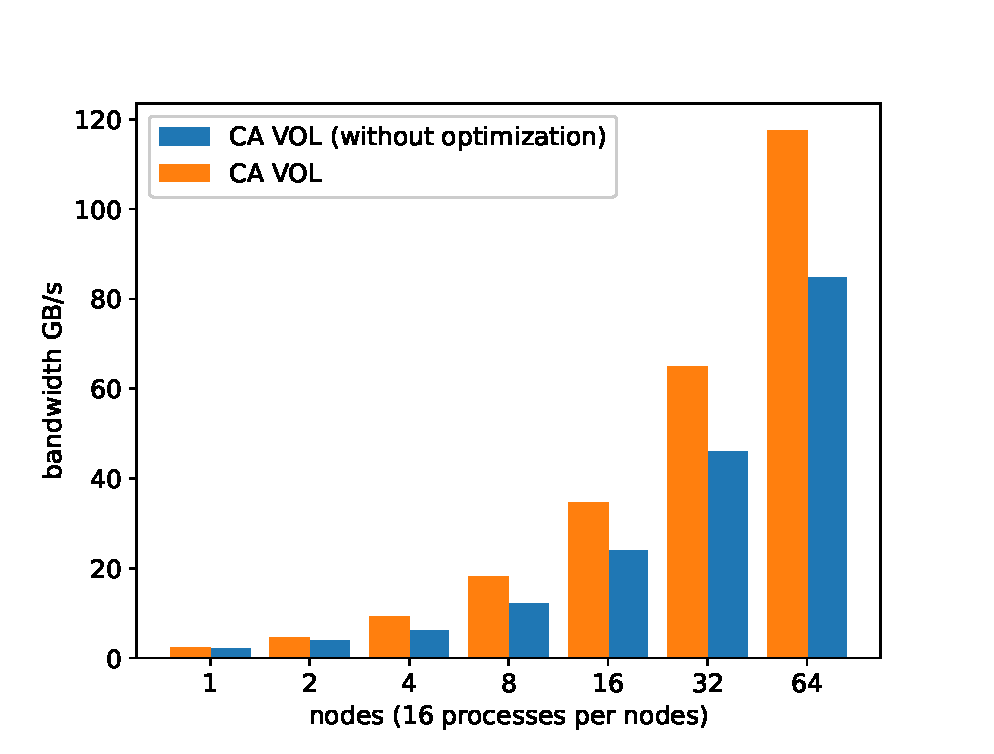
\includegraphics[width=\linewidth]{figure/chfs_strided.eps}
	\caption{h5bench writeのDIM\_1とDIM\_2を4096,4096にして,ノード数を1から64まで変化させたときのdivide volとlustreのバンド幅}
	\label{fig:h5writechfslustre}
\end{figure}


\begin{figure}[t]
	\centering
	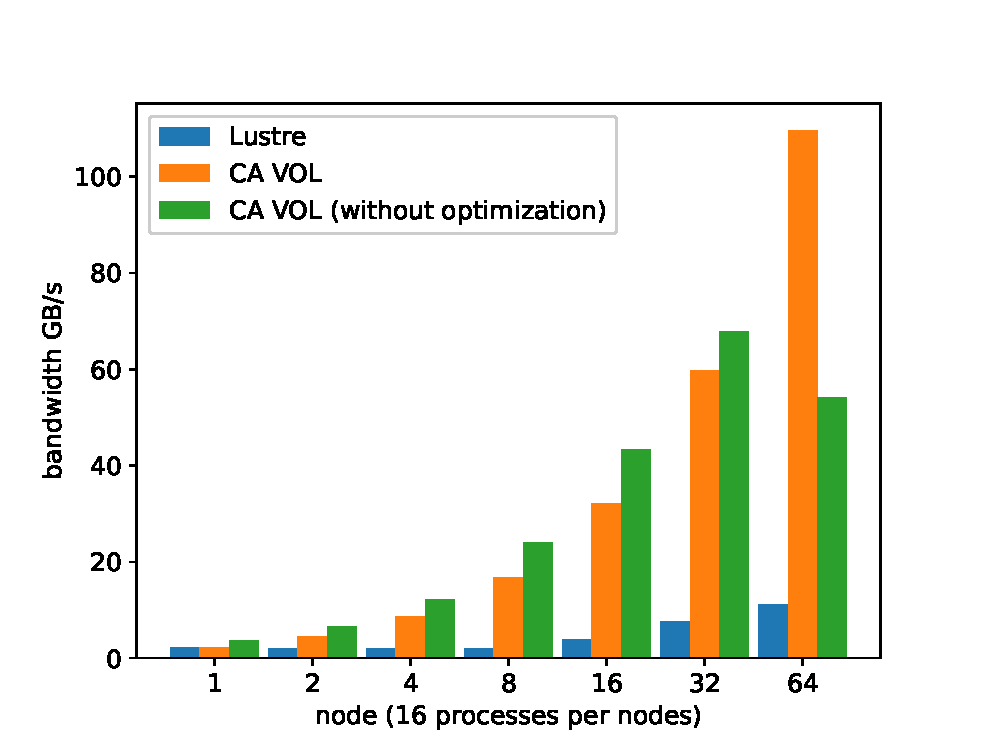
\includegraphics[width=\linewidth]{figure/segmented_chfs.eps}
	\caption{h5bench writeのDIM\_1とDIM\_2を4096,4096にして,ノード数を1から64まで変化させたときのdivide volとlustreのバンド幅}
	\label{fig:h5writechfslustre}
\end{figure}

\figref{fig:h5writechfslustre}に示すように,divide volのバンド幅はノード数を増やすごとに増加している.
64ノードではdivide volのバンド幅がlustreのバンド幅の約10倍程度となっている.
コンテキストを活用し,書き込みサイズに基づいてチャンクサイズを決定することで,
I/Oの高速化を実現できた.

\section{まとめ}
本研究では,計算性能に対してI/O性能が追いついていない問題に対して,
高レベルI/Oライブラリで得ることのできる書き込みコンテキストを利用することによるI/Oの最適化
の可能性を示した.

高レベルI/Oライブラリ経由で書き込まれるデータの粒度と
ストレージの最下層の操作単位であるオブジェクトのサイズ,チャンクサイズやストライプサイズは一致していないことが多い.
また,仮にデータの書き込みの粒度とチャンクサイズ等が等しくても,
ファイルの中でのデータの配置のアライメントの関係で,複数のプロセスから同時に同じ領域に書き込んでしまい.
その部分での並列度が失われる.
アプリケーションユーザーはこのような低層のストレージの特性を意識することなく,
高いI/O性能を得ることが望ましい.

高レベルI/Oライブラリでの抽象化レイヤー,Virtual Object Layerにおいて得ることのできる
データセットの書き込み粒度を利用する.
そのデータセットの書き込みに対して最適なチャンクサイズを決定することで,書き込みの高速化を確認した.

ストレージ階層が複雑化し,その各ストレージの性能を最大限活かすためにはこのような
高レベルI/Oライブラリで得ることのできる書き込みコンテキストを活用することが重要である.

\begin{acknowledgment}
	本研究の一部は,JSPS科研費22H00509,
	国立研究開発法人新エネルギー・産業技術総合開発機構(NEDO)
	「ポスト5G情報通信システム基盤強化研究開発事業」(JPNP20017)委託事業,
	文部科学省「次世代計算基盤に係る調査研究」事業,
	筑波大学計算科学研究センター学際共同利用プログラム,
	および富士通との特別共同研究の結果得られたものです.
\end{acknowledgment}

\bibliographystyle{ipsjsort}
\bibliography{references}

\end{document}
